\documentclass{article}
%\documentclass[twocolumn]{article}
\usepackage[utf8]{inputenc}
\usepackage[spanish]{babel}
\usepackage{graphicx}
\usepackage{verbatim}
\usepackage{moreverb}
\usepackage{amsmath}
\usepackage{amsfonts}
\usepackage{amssymb}    
\usepackage{fancybox}
\usepackage{float}
\usepackage{fancyvrb}
\usepackage{color}
\usepackage{hyperref}
\usepackage{subfigure}
\usepackage{multicol}
\numberwithin{equation}{section}
\usepackage[a4paper, hmargin=2cm, vmargin=2.5cm]{geometry}
%\usepackage[a4paper, hmargin=1.5cm, vmargin=2.5cm]{geometry}
\usepackage[retainorgcmds]{IEEEtrantools}
\usepackage{courier}
\usepackage[compact]{titlesec}

\setlength{\columnsep}{0.75cm}
%\setlength{\parskip}{0pt}

%Nuevo comando: Inserta una línea recta.
\newcommand{\HRule}{\rule{\linewidth}{0.5mm}}

%\titlespacing{\section}{0pt}{*0}{*0}
%\titlespacing{\subsection}{0pt}{*0}{*0}
%\titlespacing{\subsubsection}{0pt}{*0}{*0}


\begin{document}

%%%%%%%%%%%%%%%%%%%%%%%%%%%%%%%%% PORTADA %%%%%%%%%%%%%%%%%%%%%%%%%%%%%%%%%%%%%%

\begin{center}

{ \LARGE \bfseries Análisis de la interacción entre Pseudopercis semifasciata y Haleaeulurus bivius mediante el modelo Lotka-Volterra-Ancona}\\[0.4cm]
\large Autores: \\
\large Rezk, Mariano (mrezk@alu.itba.edu.ar)\footnote{Departamento de Ingeniería Informática del Instituto Tecnológico de Bs. As.}\\
\large Liss, Guillermo (gliss@alu.itba.edu.ar)$^1$  \\
\large Aráoz, Manuel (maraoz@alu.itba.edu.ar)$^1$  \\
\large Jardi Bello, Yemel Angel (yjardibe@alu.itba.edu.ar)$^1$ \\

\vspace{0.5cm}

% La fecha queda abajo.
{\large \today}

\end{center}

%%%%%%%%%%%%%%%%%%%%%%%%%%%%%%%%%%%%%%%%%%%%%%%%%%%%%%%%%%%%%%%%%%%%%%%%%%%%%%%%

% Seteo marcos para lo que esté en el entorno verbatim
\fvset{frame=single}

\begin{abstract}
\noindent En el presente artículo se comentan los resultados de simular la interacción predador-presa, basado en el modelo propuesto
por Lotka-Volterra-Ancona. Se ajusta un parámetro del modelo a partir de muestras experimentales y los demás parámetros bióticos, 
y luego se analizan las condiciones de estabilidad del modelo. También se estudia la influencia de los distintos parámetros
del modelo en su comportamiento, se obtiene una simplificación lineal del modelo para poblaciones cercanas al equilibrio,
y se elaboran conclusiones.

\end{abstract}


{\bf Palabras clave:} modelo presa-predador, Lotka-Volterra-Ancona, simulación de sistemas
\begin{multicols}{2}

\section{Introducción}
La especie Salmón de Mar (Pseudopercis semifasciata), es capturada en actividades pesqueras desde una latitud correspondiente a la desembocadura del Río Colorado, hasta el Golfo de San Julián. El Tiburón Pintarrojo (Haleaeulurus bivius) es una de las cincuenta especies que habitan la Plataforma Continental Argentina y preda al Salmón de Mar. La interacción presa-predador de Pseudopercis semifasciata y Haleaeulurus bivius puede modelarse mediante el modelo de Lotka-Volterra-Ancona \cite{libro}, de la forma:

\begin{equation}
\label{lva-model1}
\dot x = \lambda x - a x y
\end{equation}
\begin{equation}
\label{lva-model2}
\dot y = b x y - \mu y
\end{equation} \\

En la sección \ref{analysis} se analiza el modelo planteado, en la sección \ref{puntoa} se ajusta numéricamente el valor del parámetro $\mu$ en función de datos de muestreo, 
en la sección \ref{puntob} se analizan las condiciones de estabilidad del modelo, en la sección \ref{puntoc} se analiza la influencia de las tasas de crecimiento en el período de la evolución poblacional, y finalmente en la sección \ref{puntod} se obtiene un modelo lineal simplificado para poblaciones cercanas a las de equilibrio.

\section{Análisis del modelo}
\label{analysis}
El modelo que se utiliza para estudiar la interacción entre Pseudopercis semifasciata y Haleaeulurus bivius es determinista, dinámico y continuo. Es determinista ya que ninguno de los parámetros es una variable aleatoria, dinámico porque los valores de salida dependen de valores pasados de la entrada, y continuo ya que no se trata de una recurrencia sino de una ecuación diferencial. \\
Además, el modelo considera los efectos de los encuentros entre presa y predador, siendo el crecimiento independiente de estos. Así mismo el modelo contempla pesca y migraciones dentro de las tasas de crecimiento, pero en forma limitada ya que los términos que las contienen son lineales.

\section{Ajuste numérico del parámetro $\mu$}
\label{puntoa}
\par Conociendo los valores de los parámetros $a = 0.02yr^{-1}$ , $b = 0.035yr^{-1}$ y $\lambda = 1.5yr^{-1}$ , se utiliza el modelo ya mencionado para estimar el valor del parámetro $\mu$. Primero, se reescribe el sistema de ecuaciones diferenciales \ref{lva-model1} y \ref{lva-model2} con la notación diferencial resultando en:

\begin{equation}
\label{lva-model-d1}
\dfrac{d x}{d t} = \lambda x - a x y
\end{equation}
\begin{equation}
\label{lva-model-d2}
\dfrac{d y}{d t} = b x y - \mu y
\end{equation}

Del despeje de $d t$ y la igualación de las ecuaciones \ref{lva-model-d1} y \ref{lva-model-d2} se obtiene:

\begin{align}
ay - \lambda \ln y +bx = \mu \ln x + c
\end{align}

Haciendo el cambio de variable $z = ay - \lambda \ln y + bx$, la ecuación puede escribirse de la forma $z = Ax$ :
\begin{equation}
z = \mu x + c 
\end{equation}

Siendo la matriz de diseño $A \in \mathbb{R} ^ {n\times 2}$ para el ajuste de parámetros por el método de los cuadrádos mínimos:\\
\begin{equation}
A = \left( \begin{array}{cc} \ln x_{1} & 1 \\ \ln x_{2} & 1 \\ \vdots & \vdots \\ \ln x_{n} & 1  \end{array} \right)
\end{equation}
Aplicando dicho método se obtiene el valor de $\mu = 1.8732$ que mejor ajusta los datos históricos para los parámetros fijados. En la Figura \ref{comp_x_y} (arriba) se compara el histórico de muestreos contra la simulación realizada utilizando el valor de $\mu$ estimado y las mismas poblaciones iniciales. En la misma se observa que el ajuste se adecua a los datos y el mayor error se presenta en dónde las poblaciones toman sus máximos y mínimos. Esto último puede apreciarse también en la Figura \ref{comp_x_y} (abajo) que representa los residuos del ajuste por el método LS.

\begin{figure}[H]
\centering
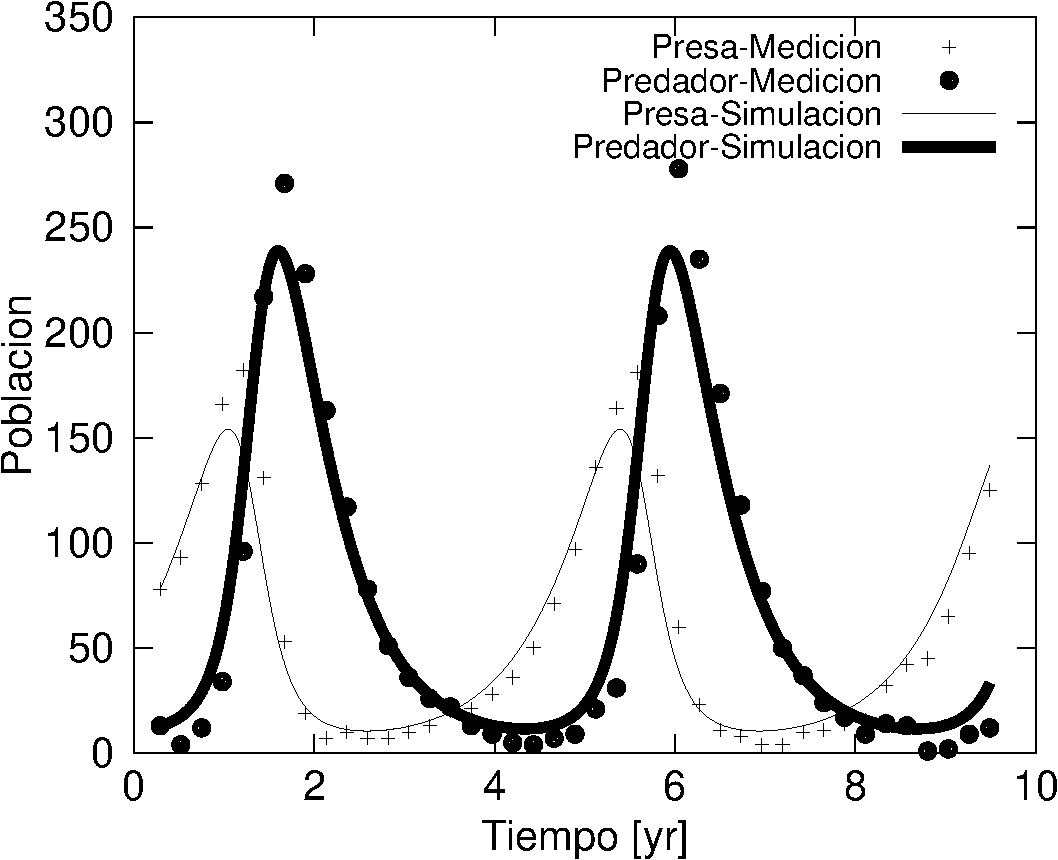
\includegraphics[width=8cm]{images/a1} \
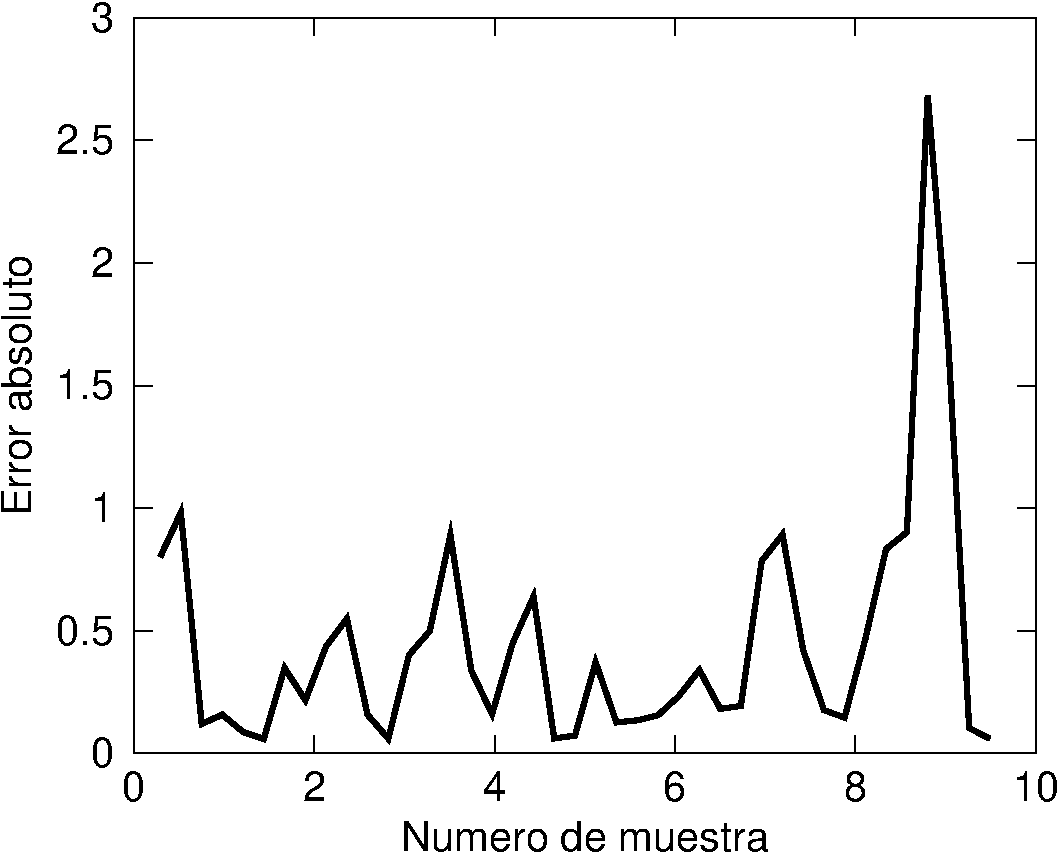
\includegraphics[width=8cm]{images/a3-bis} \
\caption{Comparación entre el histórico poblacional y la simulación del modelo (arriba). Residuos del método de resolución de cuadrádos mínimos al realizar el ajuste (abajo).}
\label{comp_x_y}
\end{figure}

En la Figura \ref{trayectoria_fase} se observan las diferencias entre el modelo y el muestreo de datos sobre el espacio de fases $x$-$y$. Las poblaciones tanto de la presa como del predador varían de forma periódica y con un desfazaje de $0.46yr$ . Este desfazaje incrementa asintóticamente hacia $0.8yr$ a medida que aumenta el valor del parámetro $a$, la razón de encuentros desfavorables para la presa. Esto último se puede observar en la Figura \ref{desfazaje}.

\begin{figure}[H]
\centering
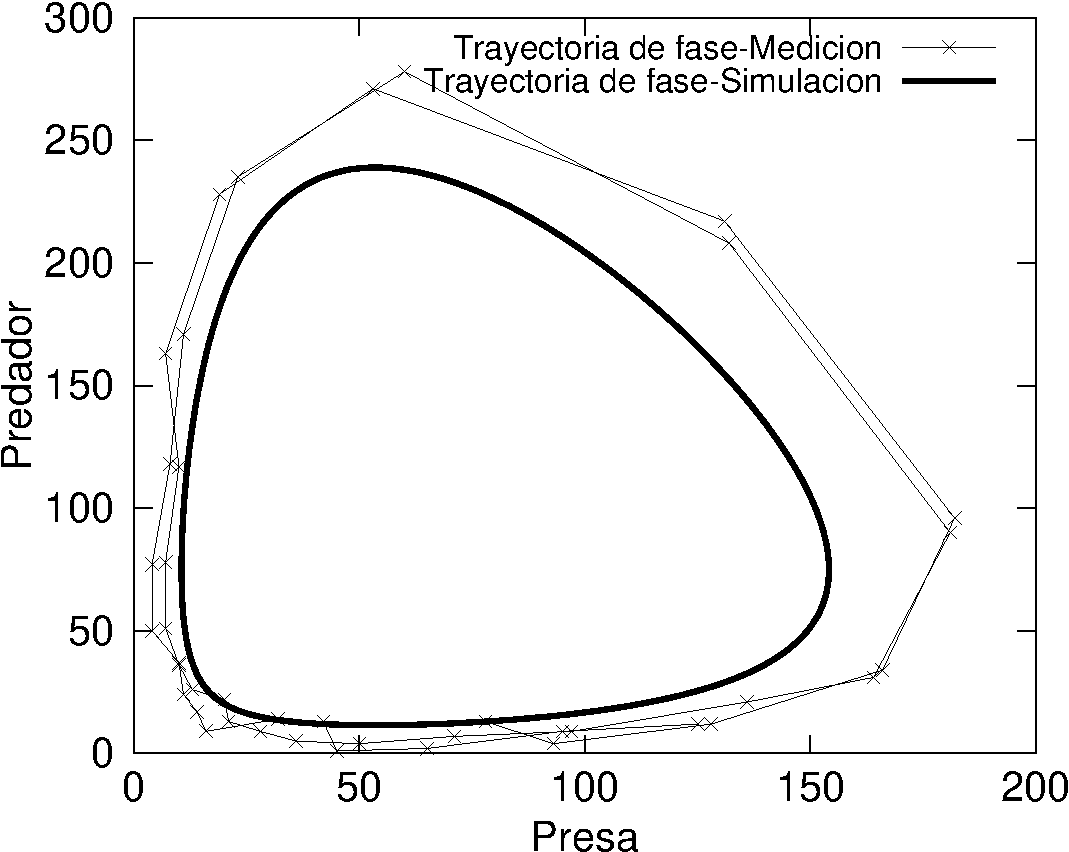
\includegraphics[width=8cm]{images/a2}
\caption{Comparación de las trayectorias de fase del modelo y los datos poblacionales.}
\label{trayectoria_fase}
\end{figure}


\begin{figure}[H]
\centering
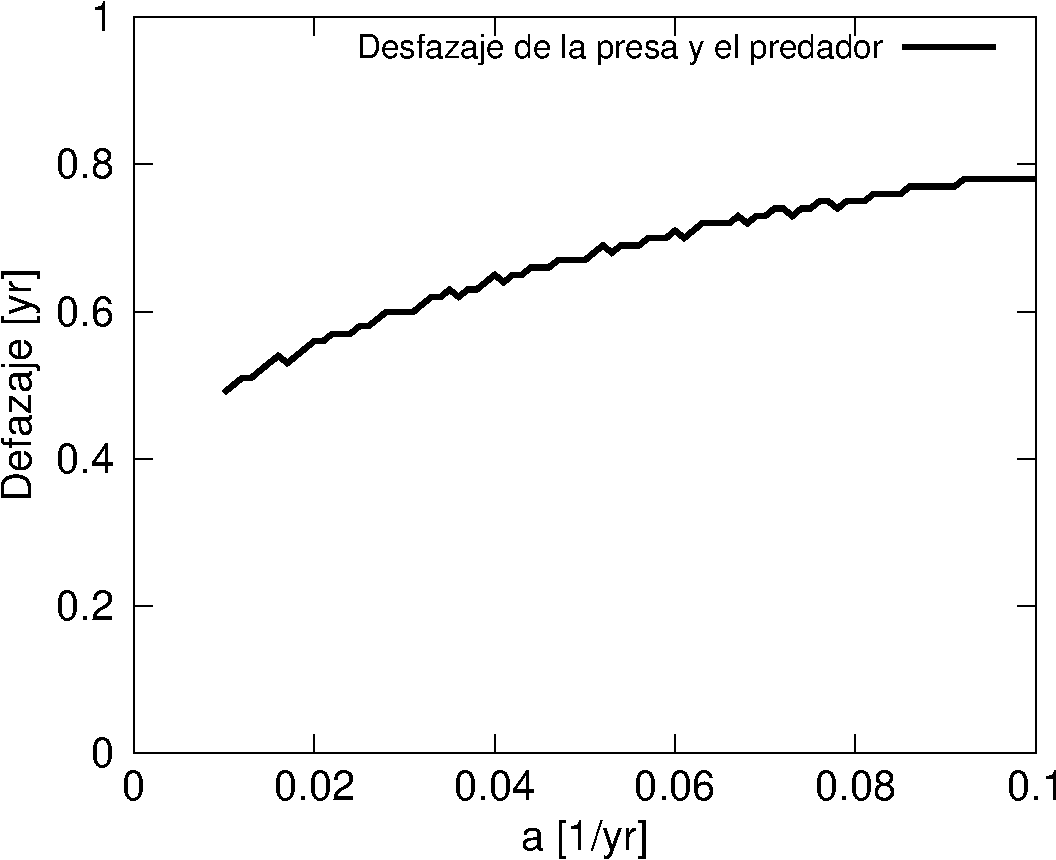
\includegraphics[width=8cm]{images/a4}
\caption{Desfazaje entre los ciclos poblacionales de la presa y el predador.}
\label{desfazaje}
\end{figure}

\begin{comment}
\end{comment}

\section{Análisis de equilibrio}
\label{puntob}    

Para hallar las poblaciones de equilibrio, se deben encontrar las poblaciones $x$ e $y$ tales que $\dot x = \dot y = 0$. 
Entonces, factorizando las ecuaciones \ref{lva-model1} y \ref{lva-model2}:

\begin{equation}
0 = x(\lambda - a y)
\end{equation}
\begin{equation}
0 = y(b x - \mu)
\end{equation}

De lo que se obtienen las dos soluciones que corresponden a poblaciones de equilibrio, y que son los pares $(x,y) \in \{(0,0),(\dfrac{\mu}{b},\dfrac{\lambda}{a})\}$. Para los datos dados y estimados, el segundo punto corresponde al par $(53,75)$. \\
Siendo $x_0$ e $y_0$ los valores iniciales de las poblaciones de presas y predadores respectivamente, se puede demostrar de forma empírica, simulando con valores de $x_0$ e $y_0$ cercanos a $(0,0)$, que el punto en cuestión es inestable. Se puede ver en la Figura \ref{equilibrio_00} como evoluciona para valores iniciales $(3,3)$ en 2 años, y analizando los valores de ambas poblaciones se observa que en el pasar de un año la población de predadores es menor que $1$ individuo, por lo que se considera a la especie como extinta en ese punto. \\

\begin{figure}[H]
\centering
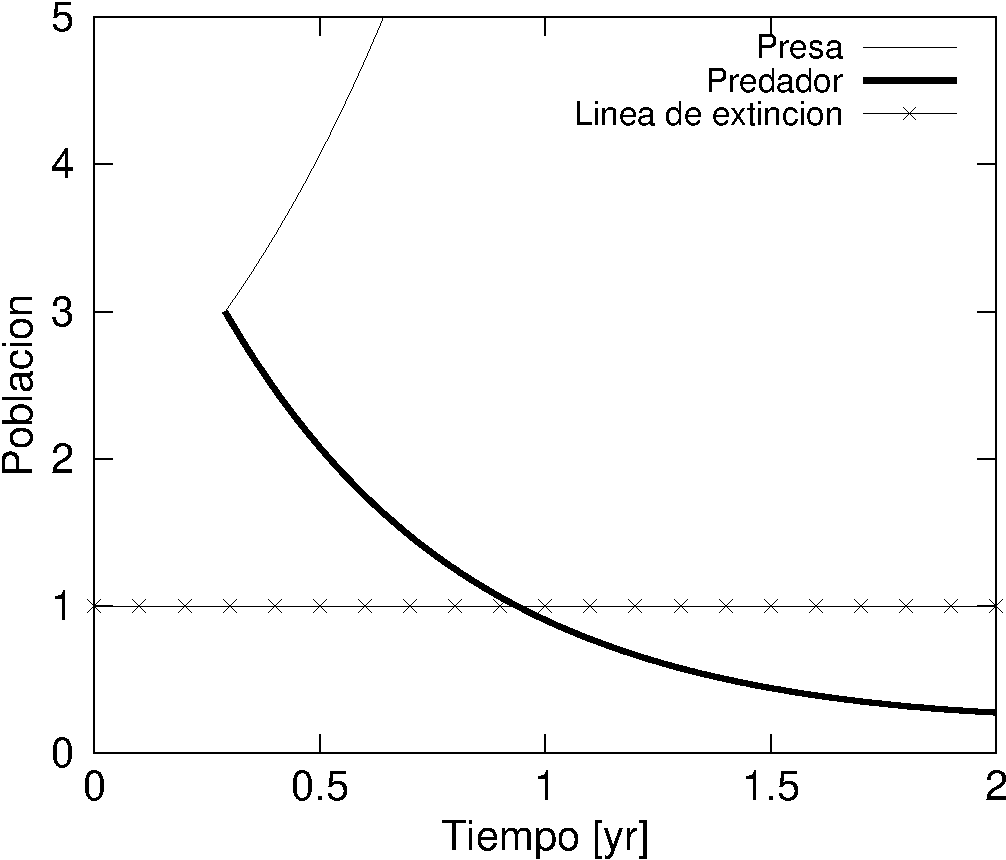
\includegraphics[width=8cm]{images/b1}
\caption{Simulación con valores iniciales de las poblaciones en (3,3).}
\label{equilibrio_00}
\end{figure}

\begin{figure}[H]
\centering
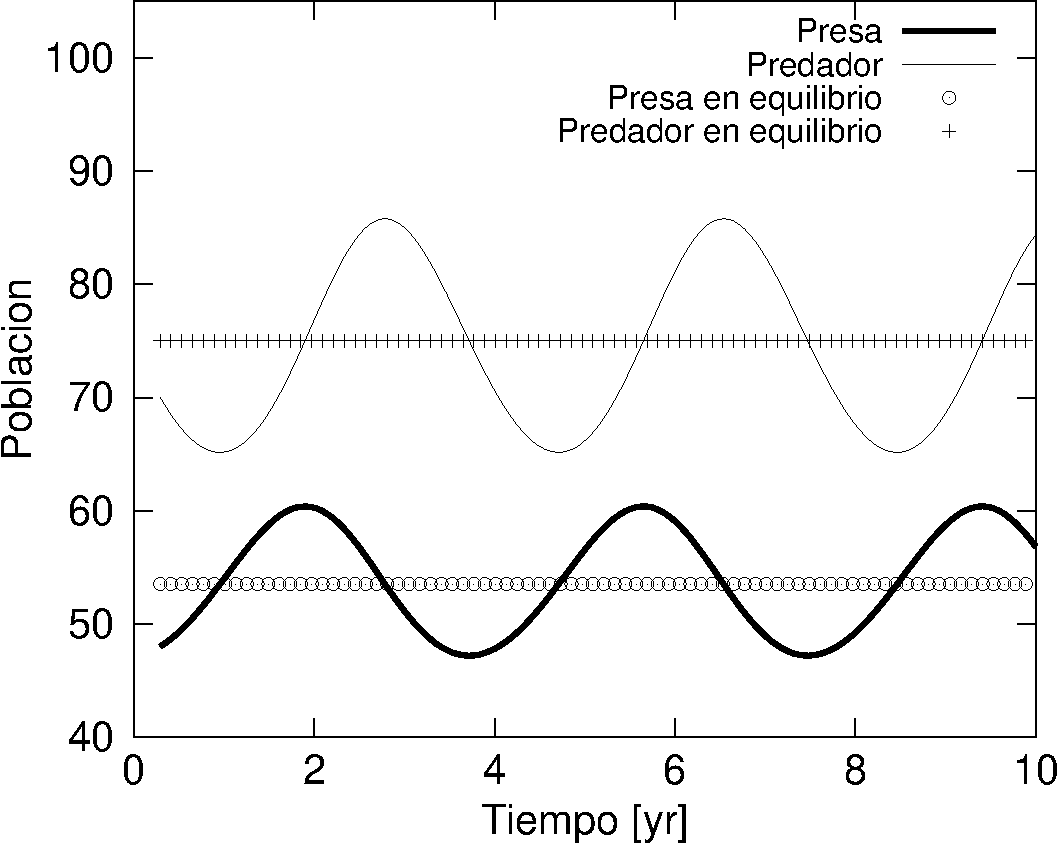
\includegraphics[width=8cm]{images/b2}
\caption{Simulación con valores de $x_0$ e $y_0$ corridos en 5 individuos con respecto al equilibrio.}
\label{equilibrio_55}
\end{figure}


En la Figura \ref{equilibrio_55} se puede ver como evoluciona el modelo para pequeños apartamientos del punto de equilibrio $(\dfrac{\mu}{b},\dfrac{\lambda}{a})$ en 10 años. Se puede observar como las poblaciones oscilan alrededor del punto de equilibrio para valores de $x_0$ e $y_0$ con un corrimiento de $5$ individuos con respecto a los valores de equilibrio, por lo que se concluye que se trata de un punto de equilibrio estable. \\


Con el objetivo de encontrar valores de $x_0$ e $y_0$ que produjeran la extinción de las especies, se simula el sistema con distintos valores de dichos parámentros. Se puede apreciar en el Cuadro \ref{table:cota_pred}, para cada valor de $x_0$, las cotas superiores aproximadas de $y_0$ tal que las poblaciones no se extinguen.


\begin{table}[H]
\center
\begin{tabular}{|c|c|}
\hline
\# presas & \# predadores \\
\hline
2 & $ 160$ \\
\hline
3 & $ 200$ \\
\hline
4 & $ 250$ \\
\hline
5 & $ 280$ \\
\hline
6 & $ 300$ \\
\hline
10 & $ 360$ \\
\hline
20 & $ 420$ \\
\hline
\end{tabular}
\caption{Cota superior aproximada del valor de $y_0$ para distintos valores de $x_0$ para los cuales no se extingan las especies}
\label{table:cota_pred}
\end{table}

\section{Análisis de influencia de los parámetros $\lambda$ y $\mu$ en el período de la evolución poblacional}
\label{puntoc}
Para medir la variación del período de las poblaciones en función de los parámetros $\lambda$ y $\mu$ se realizan dos series de simulaciones. En cada una de ellas se varía el parámetro de estudio dentro de un rango arbitrario ([1,2.3] para $\lambda$, [1.2, 2.5] para $\mu$). Tras cada simulación, comenzando con poblaciones próximas al equilibrio, se computa el período para formar las Figuras \ref{variacion_periodo_lambda} y \ref{variacion_periodo_mu}. En esta se observa que las poblaciones de presas y predadores mantienen el mismo período y este decae con el aumento $\lambda$ y $\mu$.


\section{Linealización del modelo}
\label{puntod}
Como se detalla de la sección \ref{puntob}, la población de equilibrio corresponde a los valores $(x,y) \in \{(0,0),(\dfrac{\mu}{b},\dfrac{\lambda}{a})\}$.
Sean las poblaciones de equilibrio $(X,Y)$, por tanto:
\begin{equation}
\label{zero1}
\dot x = 0 = \lambda X - a X Y
\end{equation}
\begin{equation}
\label{zero2}
\dot y = 0 = b X Y - \mu Y
\end{equation}

Suponiendo pequeños apartamientos de las poblaciones de equilibrio, esto es $x = X + \delta$ e $y = Y + \eta$, con $\delta(t) << 1$ y $\eta(t) << 1$, se escribe el modelo Lotka-Volterra-Ancona de las ecuaciones \ref{zero1} y \ref{zero2}, reemplazando:

\begin{equation}
\dot x = \lambda (X + \delta) - a (X + \delta) (Y + \eta)
\end{equation}
\begin{equation}
\dot y = b (X + \delta) (Y + \eta) - \mu (Y + \eta)
\end{equation}

\begin{figure}[H]
\centering
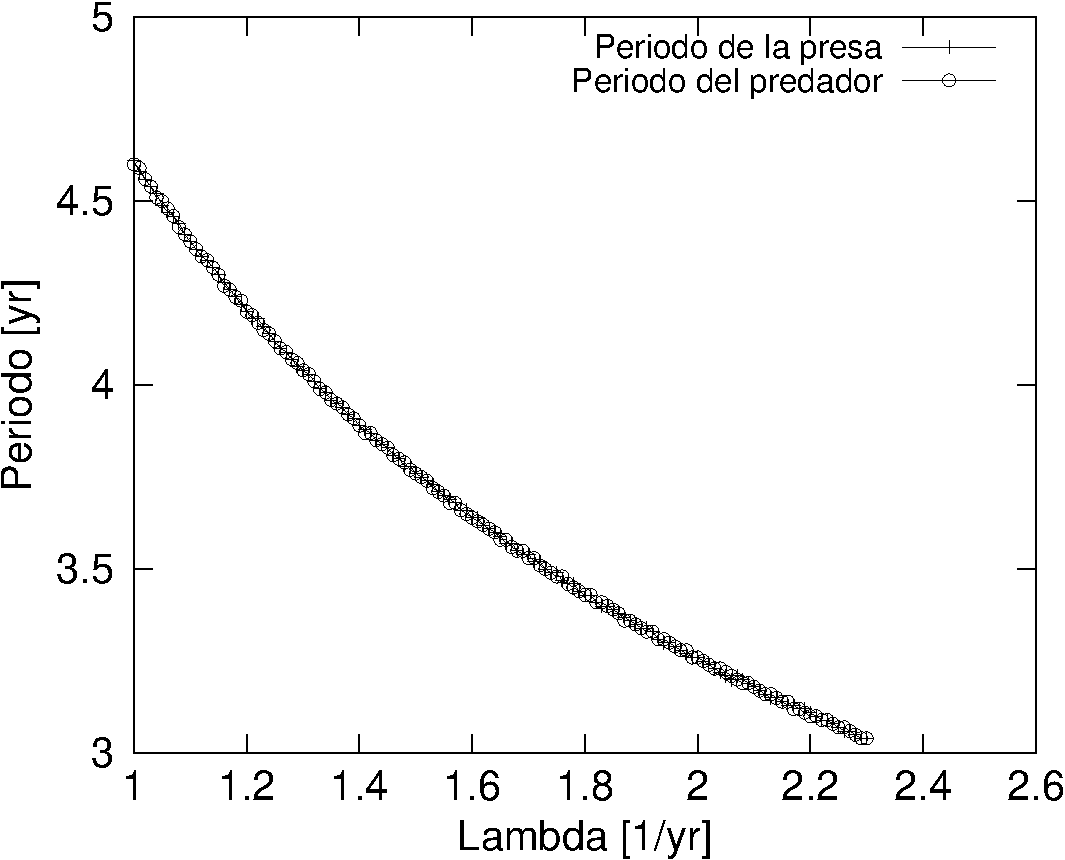
\includegraphics[width=8cm]{images/c2} \
\caption{Variación del los períodos poblacionales en función del parámetro $\lambda$.}
\label{variacion_periodo_lambda}
\end{figure}

%\begin{comment}

\begin{figure}[H]
\centering
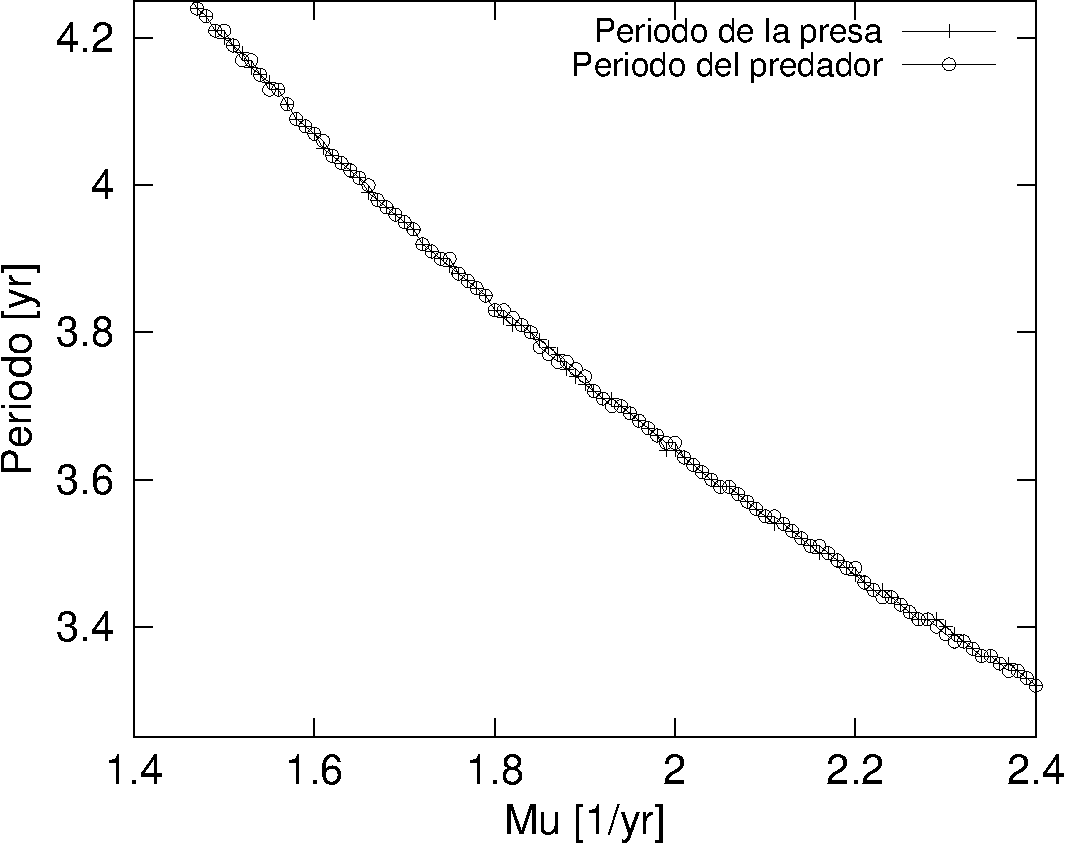
\includegraphics[width=8cm]{images/c1}
\caption{Variación del los períodos poblacionales en función del parámetro $\mu$.}
\label{variacion_periodo_mu}
\end{figure}
%\end{comment}

Al distribuir y operar se obtiene:
\begin{equation}
\dot x = (\lambda X -aXY )+ \lambda \delta - a X\eta -a Y\delta -a \delta \eta
\end{equation}
\begin{equation}
\dot y = b X\eta + bY\delta + b\delta \eta + \mu \eta +( bXY - \mu Y )
\end{equation}

A partir de \ref{zero1} y \ref{zero2} y reemplazando los valores de $X$ e $Y$ por los del punto de equilibiro $(\dfrac{\mu}{b},\dfrac{\lambda}{a})$, se obtiene:
\begin{equation}
\dot x =  - a \dfrac{\mu}{b}\eta - a \delta \eta
\end{equation}
\begin{equation}
\dot y = b\dfrac{\lambda}{a}\delta + b\delta \eta 
\end{equation}

Pero tanto $\delta$ como $\eta$ son muy pequeños, el producto $\delta \eta$ puede despreciarse, obteniendo el modelo en su versión linealizada. 
Dado que $\dot x = \dfrac{d x}{d t} = \dfrac{d (X + \delta)}{d t} = \dfrac{d \delta}{d t} = \dot \delta$, se deduce:
\begin{equation}
\label{linear1}
\dot \delta =  - a \dfrac{\mu}{b}\eta
\end{equation}
\begin{equation}
\label{linear2}
\dot \eta = b\dfrac{\lambda}{a}\delta
\end{equation}

para $\delta$ y $\eta$ pequeños apartamientos de las poblaciones de equilibrio. Este modelo corresponde a las ecuaciones de una elipse centrada en $(0,0)$. En la Figura \ref{d1} se muestra la resolución númerica de las Ecuaciones \ref{linear1} y \ref{linear2} lo que muestra que $(\dfrac{\mu}{b},\dfrac{\lambda}{a})$ es un centro y sugiere que las soluciones girarán en torno al punto de equilibrio, dando lugar, en este caso, a soluciones periódicas de las poblaciones.


\begin{figure}[H]
\centering
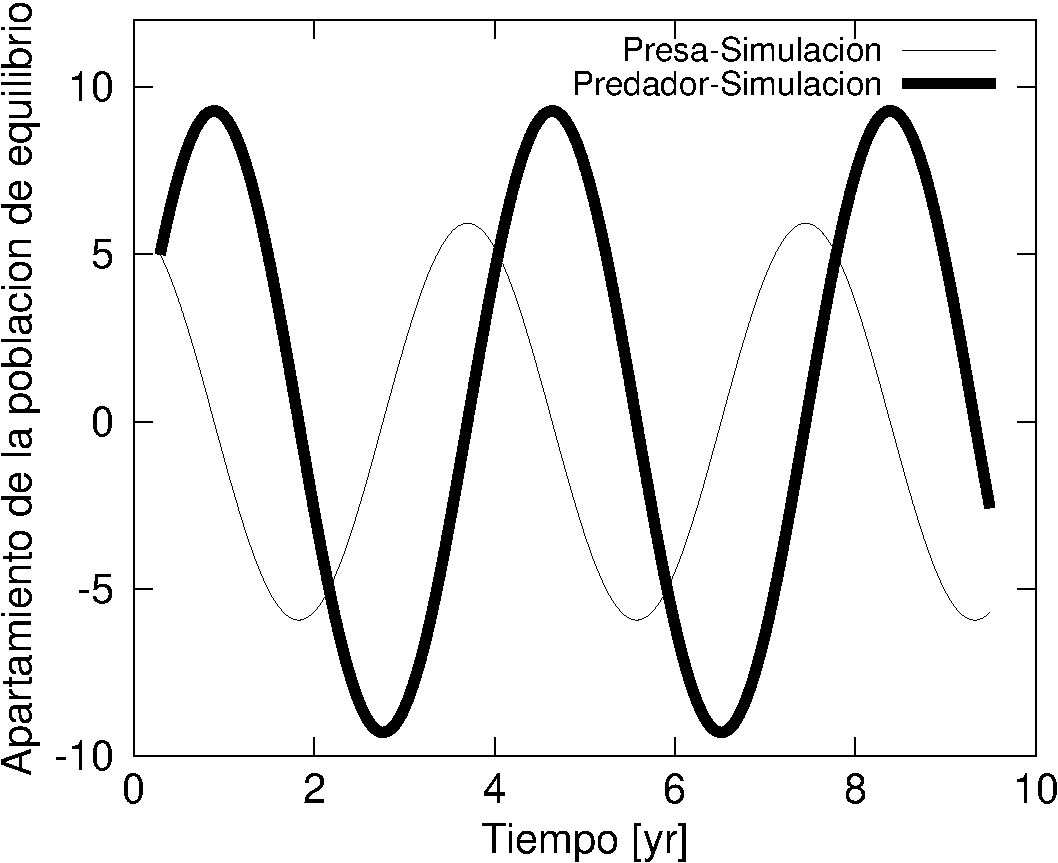
\includegraphics[width=8cm]{images/d1} \
\caption{Apartamientos del punto de equilibrio.}
\label{d1}
\end{figure}


\section{Conclusiones}
El modelo Lotka-Volterra-Ancona utilizado es simple pero limitado. Este modelo no considera relaciones con otras especies, variaciones en el clima, presencia del ser humano o la distribución espacial de los peces. Además, no toma en cuenta el sexo de los individuos para su reproducción. Tampoco considera que una población no puede crecer si cuenta con un sólo individuo, ni los efectos de la edad sobre los mismos. Sin embargo, como puede verse en la Figura \ref{comp_x_y}, el modelo ajusta los datos con considerable aptitud, ya que la curva ajustada es muy cercana a los datos de muestreo, y el error absoluto no supera el valor 3 en cada muestra.\\

En cuanto al análisis del período poblacional en función de $\lambda$ y $\mu$, se puede observar que manteniendo cualquiera de ambas constante y variando la otra, el período de ambas poblaciones (Pseudopercis semifasciata y Haleaeulurus bivius) decrece de igual forma. Esto significa que un cambio en la tasa de crecimiento o de mortandad de sólo una de las dos especies determina, según este modelo, el período de evolución $ambas$ poblaciones. El período de ambas poblaciones cae más rapidamente con el aumento de la natalidad de la presa $\lambda$ que con el aumento de la mortandad del predador $\mu$ para las simulaciones realizadas con este modelo. \\

Por último, se concluye que el modelo lineal obtenido para pequeños apartamientos de las poblaciones de equilibrio se muestra útil para poder analizar la estabilidad de estos y verificarla respecto de los resultados obtenidos empíricamente.


\begin{thebibliography}{9}
\bibitem{libro} Lotka, A.J., \emph{Analytical Note on Certain Rhythmic Relations in Organic Systems}, Proc. Natl. Acad. Sci. U.S., 6, 410-415, (1920)

\end{thebibliography}

\end{multicols}

\end{document}